\documentclass[11pt]{article}

% ── Page geometry (Letter, 1-inch margins matching the Word template) ──
\usepackage[letterpaper, margin=1in]{geometry}

% ── Font: Arial-like (Helvetica) for pdflatex ──
\usepackage[T1]{fontenc}
\usepackage{helvet}
\renewcommand{\familydefault}{\sfdefault}

% ── Packages ──
\usepackage{array}      % better table columns
\usepackage{graphicx}   % images
\usepackage{xcolor}     % colors
\usepackage{enumitem}   % list customization
\usepackage{hyperref}   % clickable links (optional)
\usepackage{tabularx}   % full-width tables
\usepackage{setspace}   % line spacing
\usepackage{listings}   
\usepackage{amsmath}
\usepackage{float}

\definecolor{codebg}{rgb}{0.96,0.96,0.94}

\lstset{
    backgroundcolor=\color{codebg},
    basicstyle=\ttfamily\footnotesize,
    keywordstyle=\color{magenta},
    numberstyle=\tiny\color{gray},
    numbers=left,
    numbersep=8pt,
    frame=none,
    breaklines=true,
    showstringspaces=false,
    tabsize=4,
    xleftmargin=1.5em,
    aboveskip=10pt,
    belowskip=10pt,
}


% ── Remove default paragraph indent, match Word spacing ──
\setlength{\parindent}{0pt}
\setlength{\parskip}{8pt}

% ── Remove page numbers (Word template has none) ──
\pagestyle{empty}

% ── Disable section numbering ──
\setcounter{secnumdepth}{0}

% ── Custom commands for template styling ──
\newcommand{\templatetitle}[1]{%
  \begin{center}
    {\fontsize{22pt}{26pt}\selectfont\textbf{\underline{#1}}}
  \end{center}
}

\newcommand{\templatesection}[1]{%
  \vspace{4pt}
  {\fontsize{14pt}{18pt}\selectfont\textbf{\underline{#1}}}
  \vspace{2pt}
}

\newcommand{\templatesubsection}[1]{%
  \textbf{\underline{#1}}
}

% ══════════════════════════════════════════════════════════════════════
\begin{document}

\templatetitle{FPGA experiment report}

Task: FPGA 3

Student 1\hspace{1.5em}name: \underline{\hspace{4cm}}\hspace{2em}ID: \underline{\hspace{3cm}}

Student 2:\hspace{1.5em}name: \underline{\hspace{4cm}}\hspace{2em}ID: \underline{\hspace{3cm}}

\vspace{6pt}

% ── Part 1 ─────────────────────────────────────────────────────────
\templatesection{Part 1 -- Status update}

Fill in the following table according to your progress at the time of the submission.

Each row should refer to one of the modules together with its simulation.

The status column should be filled with one of the following:

\begin{itemize}[nosep, leftmargin=2em]
    \item Done -- If both are written and simulation passed.
    \item Partially done -- If you started writing the module and simulation but it's not working properly.
    \item Not started -- If you didn't get to that part of the task.
\end{itemize}

When the status is \textit{partially done}, please use the notes/comments column to explain in a few more words what is the status of the module and what is the status of the simulation.

\vspace{6pt}

Fill here:

% ── Status table ──
\begin{tabularx}{\textwidth}{|X|X|X|}
\hline
Module name/Step & status & notes/comments \\
\hline
Seven Segment Display & Done & \\
\hline
Display Playground & Done & \\
\hline
Setting up constraints & Done & \\
\hline
Implementing the design & Done & \\
\hline
\end{tabularx}

\vspace{12pt}

% ── Issues ──
\templatesubsection{Issues:}

In this section please describe the current issues you are facing.

Per each module and simulation, if you receive any errors at the time of submission, please describe which errors and what they mean.

\vspace{6pt}

Fill here:

Seven Segment Display: None

Display Playground: None

Setting up constraints: None

Implementing the design: None


\newpage
% ── Part 2 ─────────────────────────────────────────────────────────
\templatesection{Part 2 -- Simulations and answers}

In this section, please add the images for each simulation as described in the report. Remember to use annotations and explain in your own words what is shown in each simulation.

In some of the tasks in the report, there are also questions that you should answer here.

Make sure to include images of all simulations running at the time of submission, even if they are not correct.

\vspace{12pt}

Fill here:

% ═══════════════════════════════════════════════════════════════
% SEVEN SEGMENT DISPLAY
% ═══════════════════════════════════════════════════════════════

\templatesubsection{Seven Segment Display:}

\vspace{6pt}

\textbf{2c. answer:}

The BASYS3 board uses a 100\,MHz clock, so the clock period is $T_{clk} = 10$\,ns. Inside the \texttt{Seg\_7\_Display} module, a 20-bit counter \texttt{clkdiv} increments on every rising clock edge. The least significant bit (LSB) toggles every 10\,ns, and in general, the $n$-th bit toggles every $10 \times 2^{n}$\,ns.

According to the experiment instructions, the total refresh time for all 4 digits must be between 1\,ms and 16\,ms. Since there are four digits, we need two bits from the counter to cycle through them (values 00, 01, 10, 11).

We chose: $s = \texttt{clkdiv}[19:18]$

Each digit selection changes every $10 \times 2^{18}\,\text{ns} = 2.62$\,ms. For all four digits, the total refresh period is:
\[
T_{refresh} = 4 \times 2.62\,\text{ms} = 10.49\,\text{ms}
\]

This satisfies the requirement $1\,\text{ms} \leq T_{refresh} \leq 16\,\text{ms}$, ensuring flicker-free display for the human eye.

\vspace{12pt}

% ═══════════════════════════════════════════════════════════════
% DISPLAY PLAYGROUND
% ═══════════════════════════════════════════════════════════════

\templatesubsection{Display Playground:}

\vspace{6pt}

\textbf{3b. answer:}

The Display Playground module architecture consists of the following functional blocks:

\begin{itemize}[nosep]
    \item \textbf{Input clamping logic:} Four parallel comparators check whether each 4-bit switch group (\texttt{sw[3:0]}, \texttt{sw[7:4]}, \texttt{sw[11:8]}, \texttt{sw[15:12]}) exceeds the value 9. If so, a multiplexer replaces the value with 9 (\texttt{4'b1001}). Otherwise the original switch value passes through.
    \item \textbf{Seg\_7\_Display instance:} The clamped 16-bit value \texttt{fixed\_sw} is fed to the \texttt{Seg\_7\_Display} module, which handles the time-multiplexed driving of the four 7-segment digits.
    \item \textbf{LED decoder:} A case statement maps the first digit (\texttt{fixed\_sw[3:0]}) to the corresponding LED (0--9), producing a one-hot encoding on the 10 LEDs.
\end{itemize}

\vspace{6pt}

\textbf{3c. answer:}

If the switches indicate a number greater than 9 (for example, \texttt{4'b1101} which equals 13 in decimal), the design clamps the value to 9, the maximum single decimal digit. This is implemented using a generate loop with comparators: for each 4-bit group, if the value exceeds \texttt{4'd9}, it is replaced by \texttt{4'd9}. This prevents undefined behavior on the 7-segment display and ensures only digits 0--9 are ever shown.

\vspace{6pt}

\textbf{3f. answer:}

\begin{figure}[H]
    \centering
    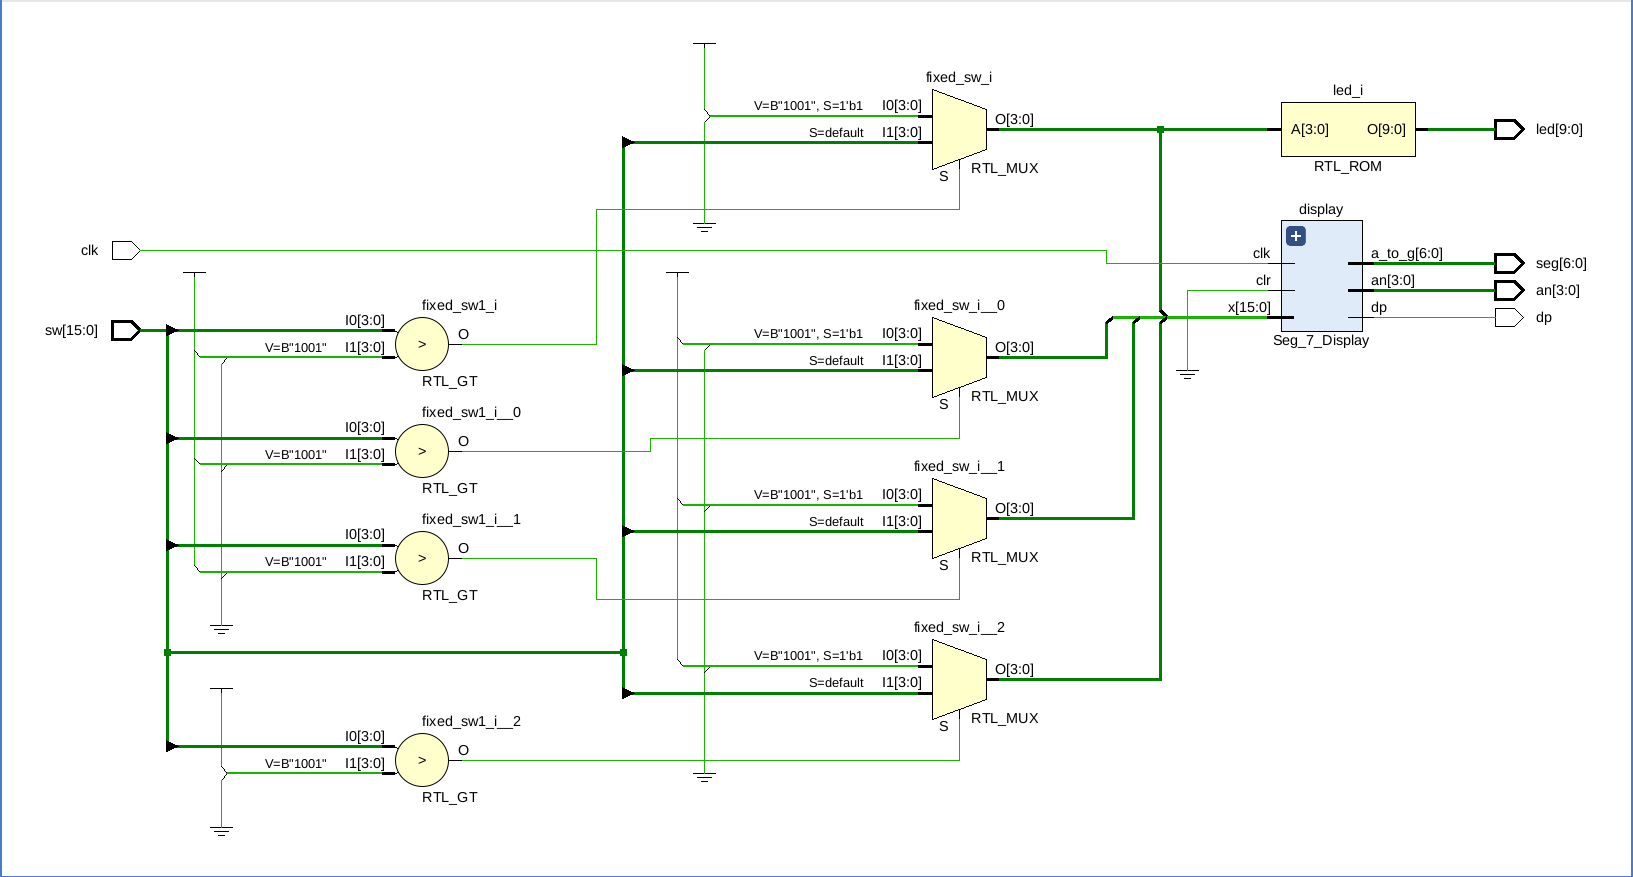
\includegraphics[width=\textwidth]{linter_des.png}
    \caption{RTL elaborated design schematic of Display\_Playground. The schematic shows four \texttt{RTL\_GT} comparators checking each 4-bit switch group against 9, four \texttt{RTL\_MUX} multiplexers selecting between the original and clamped values, an \texttt{RTL\_ROM} for the LED decoder, and the instantiated \texttt{Seg\_7\_Display} module.}
\end{figure}

\newpage
\textbf{3g. answer:}

\begin{figure}[H]
    \centering
    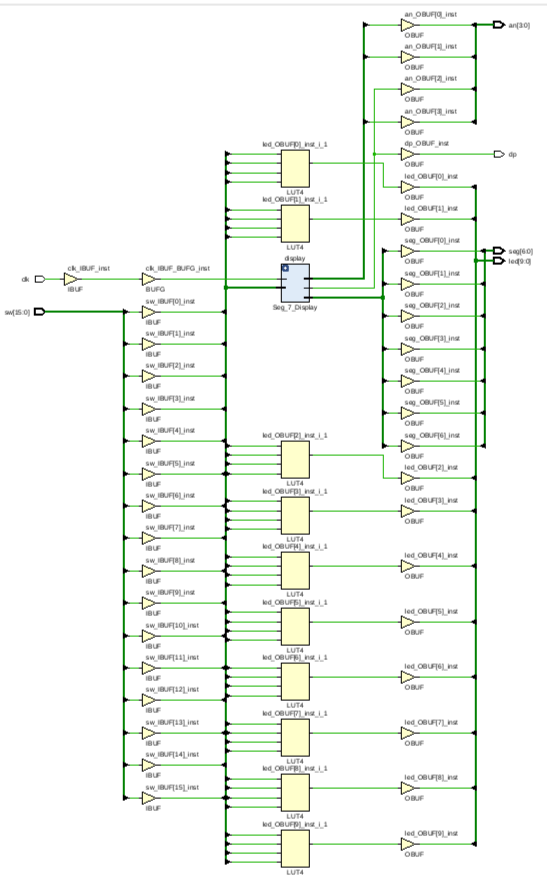
\includegraphics[width=0.55\textwidth]{synthesis_sch.png}
    \caption{Synthesized design schematic of Display\_Playground. The comparators and muxes have been optimized into \texttt{LUT4} look-up tables. Input buffers (\texttt{IBUF}) and output buffers (\texttt{OBUF}) have been inserted for the physical I/O. The clock input passes through a \texttt{BUFG} global clock buffer.}
\end{figure}

In the elaborated design we see the logical structure of the design as written in Verilog, before any optimization. We can see how modules, registers and logic blocks are connected based on the Verilog code we wrote.

In the synthesized design schematic we see the actual hardware resources that the FPGA will use to implement the Verilog code. The high-level constructs (comparators, multiplexers, ROM) are mapped to FPGA primitives such as \texttt{LUT4} look-up tables, and I/O buffer primitives (\texttt{IBUF}, \texttt{OBUF}, \texttt{BUFG}) are inserted for all external connections.

\vspace{12pt}

% ═══════════════════════════════════════════════════════════════
% SETTING UP CONSTRAINTS
% ═══════════════════════════════════════════════════════════════

\templatesubsection{Setting up constraints:}

\vspace{6pt}

The constraints file \texttt{fpga\_lab\_constraints.xdc} was configured as follows:

\begin{enumerate}[nosep]
    \item \textbf{Clock signal:} Uncommented the two lines connecting \texttt{clk} to pin \texttt{W5} with LVCMOS33 I/O standard.
    \item \textbf{Timing constraint:} Uncommented the \texttt{create\_clock} command specifying a 10\,ns period (100\,MHz) for \texttt{sys\_clk\_pin}.
    \item \textbf{Switch inputs:} Uncommented all 16 switch lines (\texttt{sw[0]} through \texttt{sw[15]}).
    \item \textbf{7-segment outputs:} Uncommented the 7 segment lines (\texttt{seg[0]}--\texttt{seg[6]}), the 4 anode lines (\texttt{an[0]}--\texttt{an[3]}), and the decimal point (\texttt{dp}).
    \item \textbf{LED outputs:} Uncommented 10 LED output pins (\texttt{led[0]}--\texttt{led[9]}) mapped to pins U16, E19, U19, V19, W18, U15, U14, V14, V13, and V3.
\end{enumerate}

\vspace{12pt}

% ═══════════════════════════════════════════════════════════════
% IMPLEMENTING THE DESIGN
% ═══════════════════════════════════════════════════════════════

\templatesubsection{Implementing the design:}

\vspace{6pt}

\textbf{5c. answer:}

\begin{figure}[H]
    \centering
    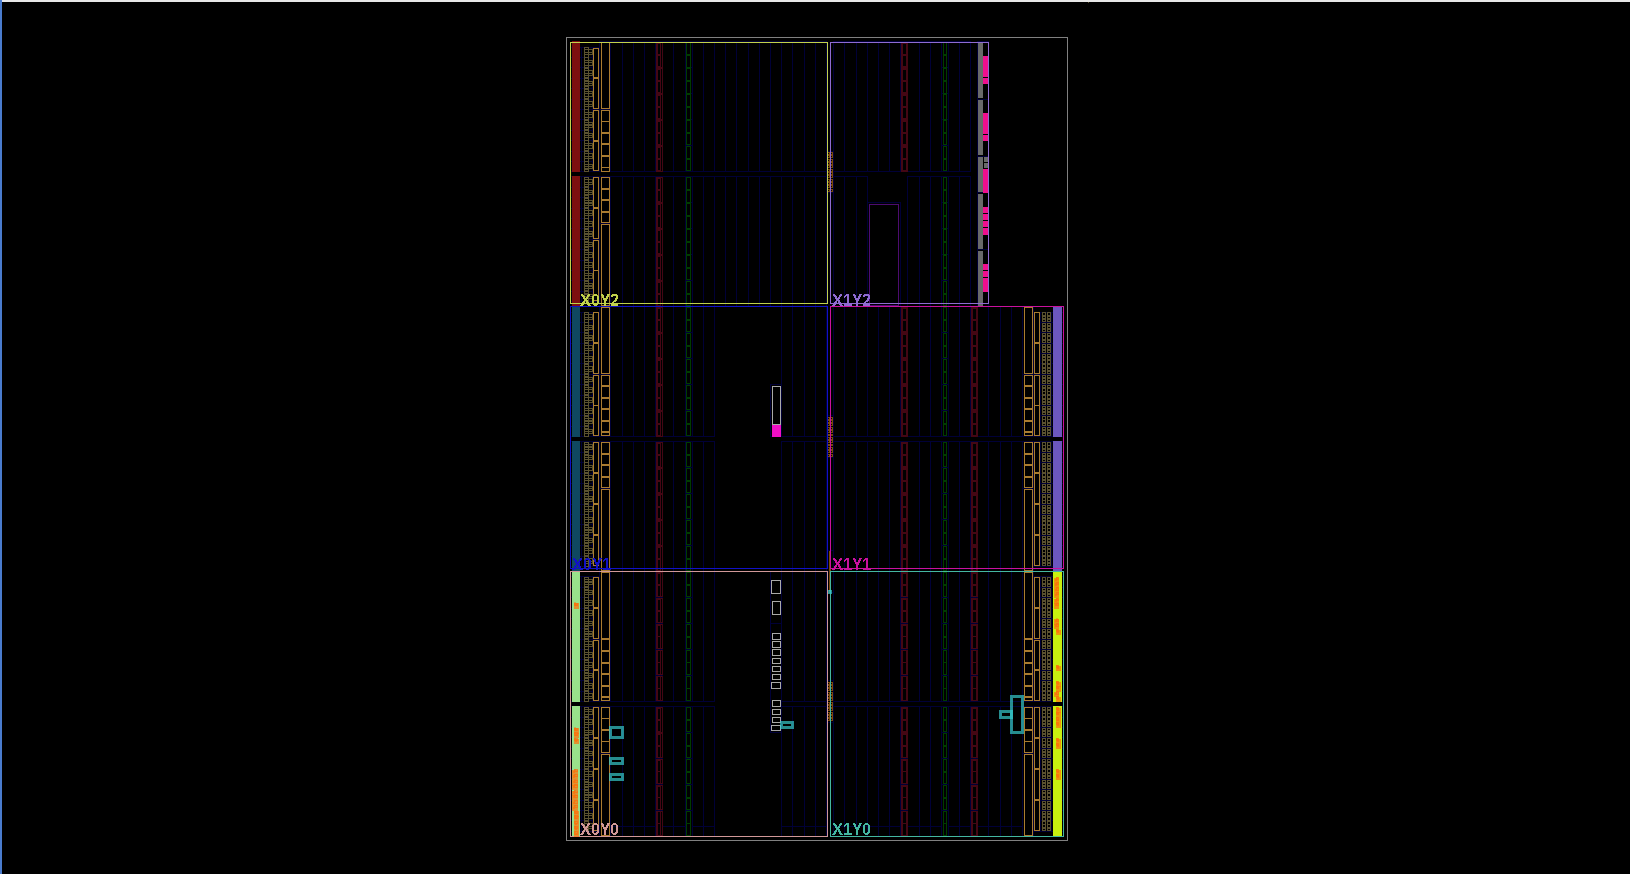
\includegraphics[width=0.85\textwidth]{implemntation_des.png}
    \caption{FPGA implementation floorplan view showing the placed and routed design on the Artix-7 device. The utilized resources are concentrated in a small region of the chip.}
\end{figure}

\newpage
\textbf{5d. answer:}

\begin{figure}[H]
    \centering
    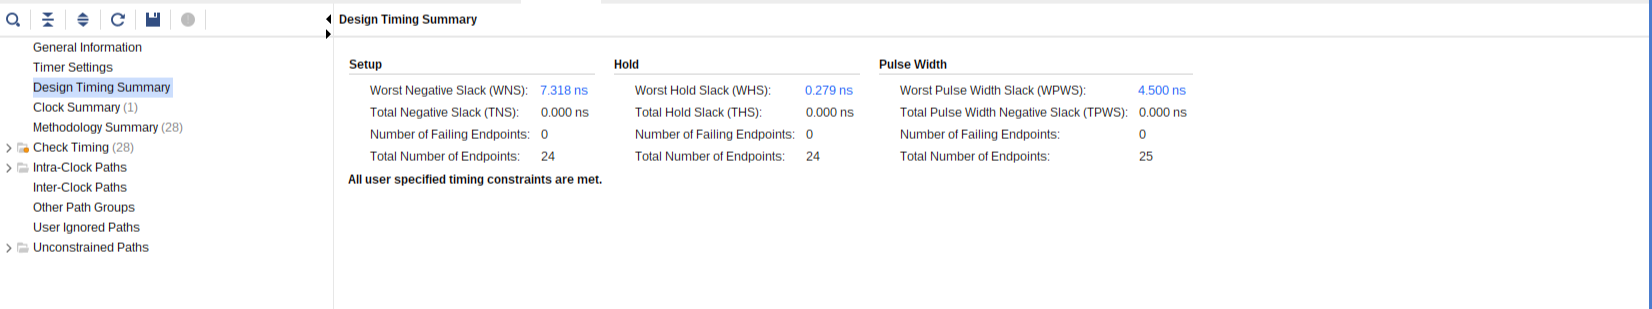
\includegraphics[width=\textwidth]{timing_rep.png}
    \caption{Design Timing Summary showing positive slack for both setup and hold times. All user-specified timing constraints are met.}
\end{figure}

The timing summary confirms:
\begin{itemize}[nosep]
    \item \textbf{Setup:} Worst Negative Slack (WNS) = 7.318\,ns (positive $\Rightarrow$ constraint met)
    \item \textbf{Hold:} Worst Hold Slack (WHS) = 0.279\,ns (positive $\Rightarrow$ constraint met)
    \item \textbf{Pulse Width:} Worst Pulse Width Slack (WPWS) = 4.500\,ns (positive $\Rightarrow$ constraint met)
    \item Number of Failing Endpoints: 0 for all categories
\end{itemize}

\vspace{6pt}

\textbf{5e. answer:}

The critical setup path length can be calculated from the worst negative slack:
\begin{align*}
\text{setup slack} &= (T_{clk}) - (T_{critical\,path}) \\
7.318 &= 10 - (T_{critical\,path}) \\
T_{critical\,path} &= 2.682\,[\text{ns}]
\end{align*}

Another way to find the critical path is from the Vivado software:

\begin{figure}[H]
    \centering
    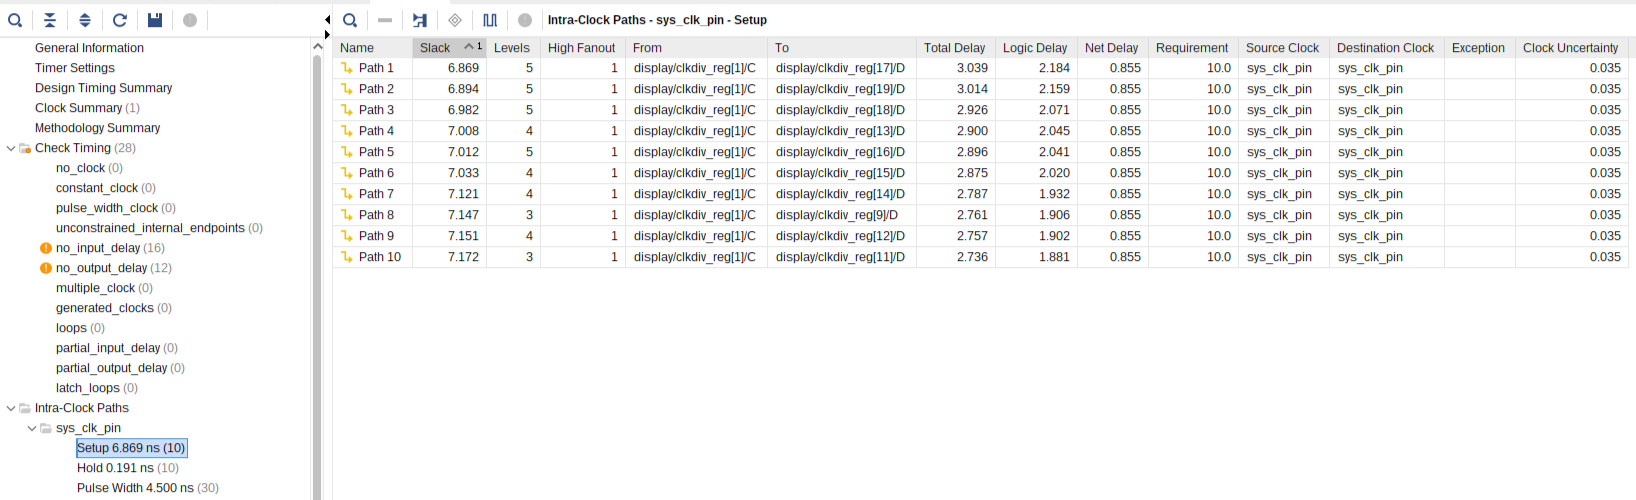
\includegraphics[width=\textwidth]{critical_path.png}
    \caption{Intra-Clock Paths showing the critical path from \texttt{display/clkdiv\_reg[1]/C} to \texttt{display/clkdiv\_reg[17]/D} with a total delay of 3.039\,ns.}
\end{figure}

We can see that the critical path is $3.039\,[\text{ns}]$ which is close to the value we calculated. The small difference is due to the inclusion of clock uncertainty (0.035\,ns) in the slack computation.

\newpage

\textbf{6a--b. Bitstream Generation and Programming:}

The bitstream was generated successfully and the design was programmed onto the BASYS3 board.

\begin{figure}[H]
    \centering
    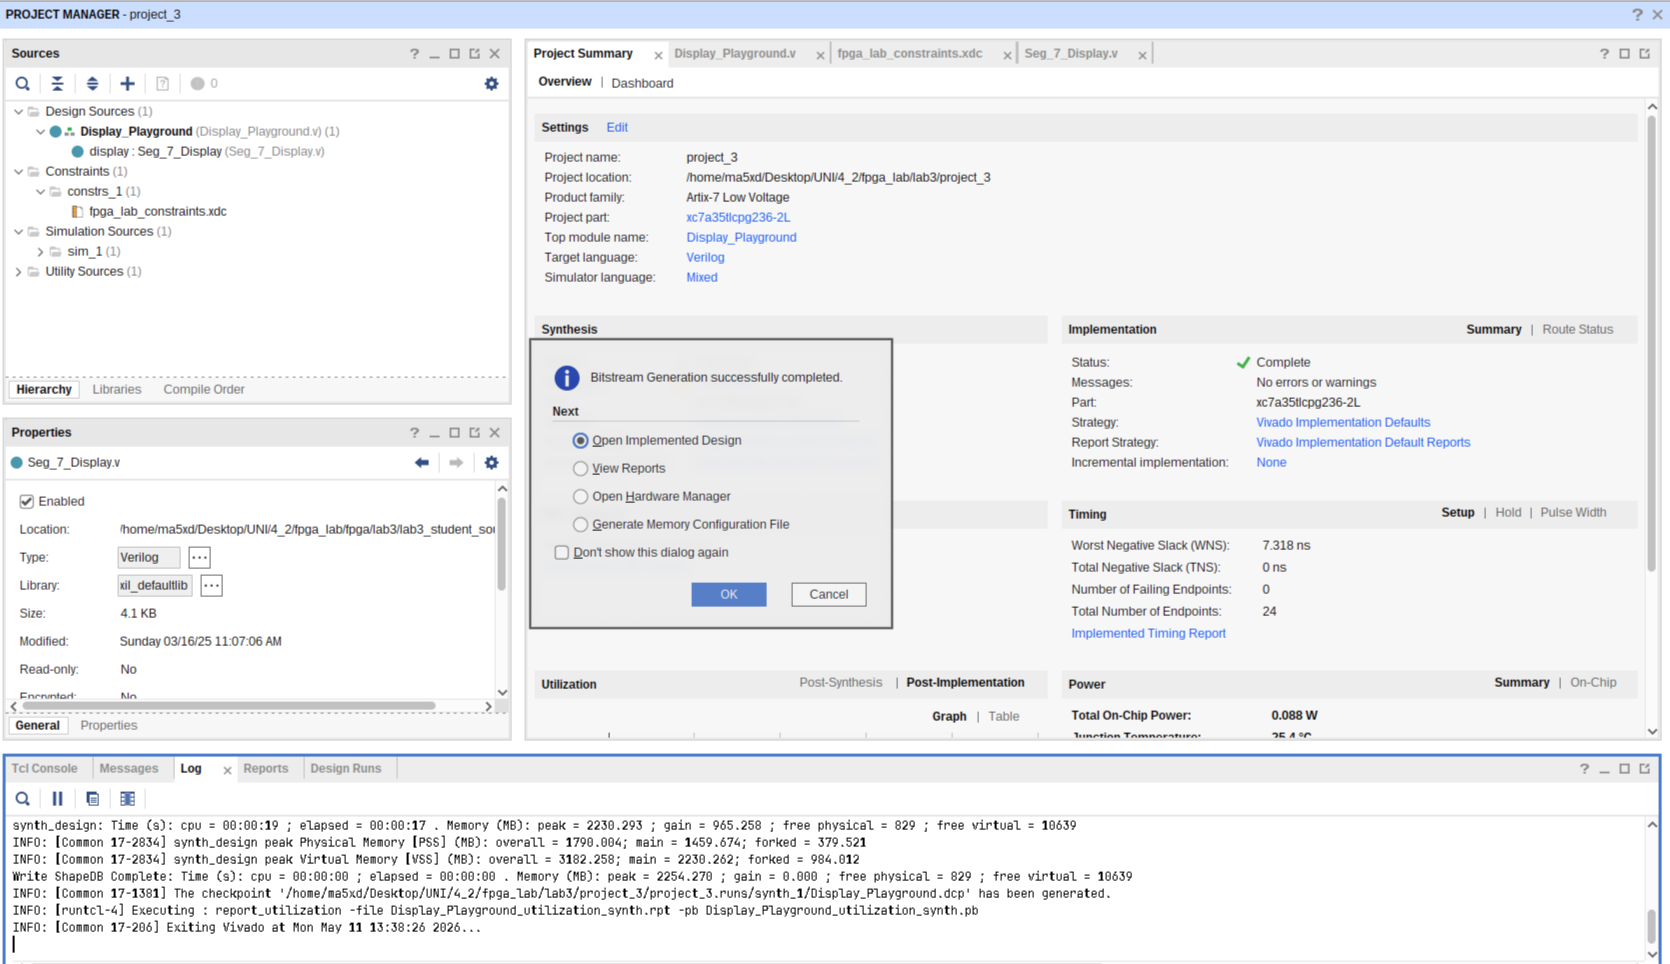
\includegraphics[width=\textwidth]{bit_stream.png}
    \caption{Project Summary showing successful bitstream generation. Implementation status is ``Complete'' with no errors or warnings. WNS = 7.318\,ns, Total On-Chip Power = 0.088\,W.}
\end{figure}

The design was verified on hardware: setting the 16 switches to represent four decimal digits correctly displayed them on the 7-segment display, and the corresponding LED for the first digit lit up.

\vspace{6pt}

\textbf{6c. answer:}

After removing the debug core and re-implementing the design:

\begin{figure}[H]
    \centering
    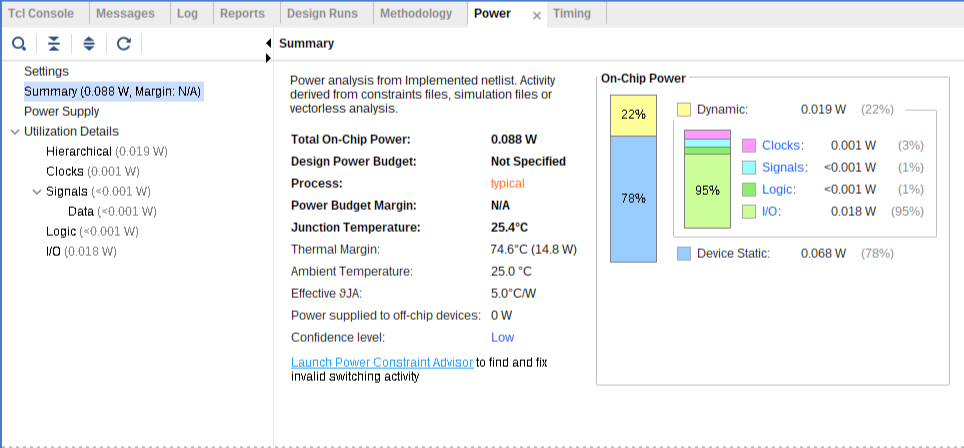
\includegraphics[width=0.85\textwidth]{power_report.png}
    \caption{Power report summary. Total On-Chip Power = 0.088\,W, consisting of 0.019\,W dynamic (22\%) and 0.068\,W static (78\%). Junction temperature = 25.4$^{\circ}$C.}
\end{figure}

\begin{figure}[H]
    \centering
    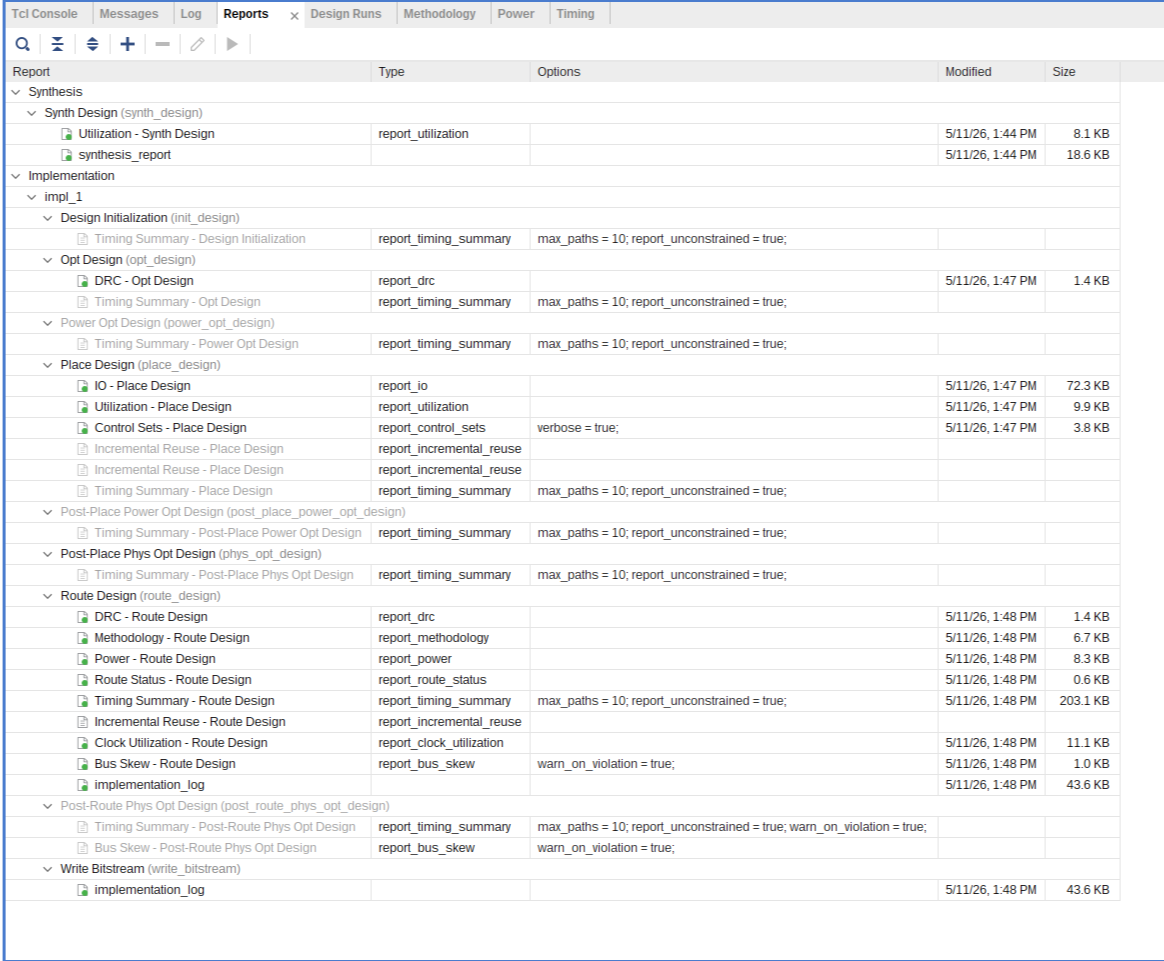
\includegraphics[width=\textwidth]{reports.png}
    \caption{Vivado Reports tab showing all synthesis and implementation reports generated successfully.}
\end{figure}

\newpage
% ═══════════════════════════════════════════════════════════════
% APPENDIX: VERILOG SOURCE CODE
% ═══════════════════════════════════════════════════════════════

\templatesection{Appendix -- Verilog Source Code}

\vspace{6pt}

Seg\_7\_Display.v

\begin{lstlisting}
`timescale 1ns/10ps
//////////////////////////////////////////////////////////////
// Company:         Tel Aviv University
// Module Name:     Seg_7_Display
// Description:     Translates input vector "x" into 7-segment
//                  display signals with time-multiplexed digits
//////////////////////////////////////////////////////////////
module Seg_7_Display(
    input [15:0] x,
    input clk,
    input clr,
    output reg [6:0] a_to_g,
    output reg [3:0] an,
    output wire dp
);

    wire [1:0] s;
    reg [3:0] digit;

    // For 100MHz clock
    reg [19:0] clkdiv = 19'b0;
    assign s = clkdiv[19:18];

    assign dp = (s == 2'b10) ? 0 : 1;

    always @(posedge clk)
        case(s)
            0: digit = x[3:0];
            1: digit = x[7:4];
            2: digit = x[11:8];
            3: digit = x[15:12];
            default: digit = x[3:0];
        endcase

    // 7-segment decoder
    always @(*)
        case(digit)
            0:  a_to_g = 7'b1000000;
            1:  a_to_g = 7'b1111001;
            2:  a_to_g = 7'b0100100;
            3:  a_to_g = 7'b0110000;
            4:  a_to_g = 7'b0011001;
            5:  a_to_g = 7'b0010010;
            6:  a_to_g = 7'b0000010;
            7:  a_to_g = 7'b1111000;
            8:  a_to_g = 7'b0000000;
            9:  a_to_g = 7'b0010000;
            'hA: a_to_g = 7'b0111111; // dash
            'hB: a_to_g = 7'b1111111; // off
            'hC: a_to_g = 7'b1110111;
            default: a_to_g = 7'b0000000;
        endcase

    // Anode selection (active low)
    always @(*) begin
        an = 4'b1111;
        an[s] = 0;
    end

    // Clock divider counter
    always @(posedge clk or posedge clr) begin
        if (clr == 1)
            clkdiv <= 0;
        else
            clkdiv <= clkdiv + 1;
    end
endmodule
\end{lstlisting}

\newpage

Display\_Playground.v

\begin{lstlisting}
`timescale 1ns/10ps
//////////////////////////////////////////////////////////////
// Company:         Tel Aviv University
// Module Name:     Display_Playground
// Description:     Top module - switches select display values,
//                  LEDs indicate first digit
// Dependencies:    Seg_7_Display
//////////////////////////////////////////////////////////////
module Display_Playground(clk, sw, seg, an, dp, led);

    input clk;
    input [15:0] sw;
    output wire [6:0] seg;
    output wire [3:0] an;
    output wire       dp;
    output reg [9:0] led;

    reg [15:0] fixed_sw;

    genvar i;
    for (i = 0; i < 4; i = i + 1) begin
        always @(*) begin
            if (sw[(i*4)+3:i*4] > 4'd9)
                fixed_sw[(i*4)+3:i*4] = 4'd9;
            else
                fixed_sw[(i*4)+3:i*4] = sw[(i*4)+3:i*4];
        end
    end

    always @(*) begin
        led = 0;
        case(fixed_sw[3:0])
            4'b0000: led[0] = 1'b1;
            4'b0001: led[1] = 1'b1;
            4'b0010: led[2] = 1'b1;
            4'b0011: led[3] = 1'b1;
            4'b0100: led[4] = 1'b1;
            4'b0101: led[5] = 1'b1;
            4'b0110: led[6] = 1'b1;
            4'b0111: led[7] = 1'b1;
            4'b1000: led[8] = 1'b1;
            4'b1001: led[9] = 1'b1;
            default: led = 0;
        endcase
    end

    Seg_7_Display display(fixed_sw, clk, 0, seg, an, dp);

endmodule
\end{lstlisting}

\end{document}
